\documentclass[11pt]{article}

\usepackage[a4paper,margin=1in]{geometry}
\usepackage{amsmath,amssymb,bm}
\usepackage{graphicx}
\usepackage{booktabs}
\usepackage{hyperref}
\usepackage{xcolor}

\hypersetup{
    colorlinks=true,
    linkcolor=blue,
    citecolor=blue,
    urlcolor=blue
}

\title{\textbf{Technical Note: FFT Spectral Leakage Using Matrix-Based DFT Analysis}}
\author{Hossein Molhem\\DSP-Array-Processing-Lab}
\date{May 19, 2026}

\begin{document}

\maketitle

\begin{abstract}
This technical note presents a matrix-based interpretation of FFT spectral leakage using the first exercise in the DSP-Array-Processing-Lab repository. The exercise compares a coherent sinusoid at 125 Hz with a non-coherent sinusoid at 123.5 Hz under a sampling rate of 1000 Hz and a record length of 256 samples. The note formulates the sampled signal as a vector, expresses the DFT as a finite DFT-basis projection, and interprets spectral leakage as a frequency-grid mismatch between the input sinusoid and the finite-dimensional DFT basis. This formulation is intended to support simulation, documentation, interview preparation, and future extensions toward windowing, spectral estimation, radar processing, and array-processing workflows.
\end{abstract}

\section{Purpose and Scope}

The purpose of this note is to provide a professional mathematical explanation of FFT spectral leakage for the repository exercise:

\begin{center}
\texttt{python/ex01\_fft\_spectral\_leakage/}
\end{center}

The implementation generates two real-valued sinusoidal signals, computes their single-sided FFT magnitude spectra, normalizes the spectra in decibels, and saves a comparison figure. This note focuses on the theoretical foundation behind that simulation.

The central engineering question is:

\begin{quote}
Why does one sinusoid produce a concentrated FFT peak, while another sinusoid spreads energy across multiple FFT bins?
\end{quote}

The answer is that the FFT evaluates a finite set of orthogonal frequency-grid basis vectors. A sinusoid aligned with one of those basis vectors is represented compactly. A sinusoid between basis vectors is represented by projections onto many DFT basis vectors, producing spectral leakage.

\section{Simulation Parameters}

The simulation uses the parameters listed in Table~\ref{tab:sim_params}.

\begin{table}[htbp]
\centering
\caption{Exercise 01 simulation parameters.}
\label{tab:sim_params}
\begin{tabular}{ll}
\toprule
Parameter & Value \\
\midrule
Sampling rate & $f_s = 1000$ Hz \\
Number of samples & $N = 256$ \\
FFT bin spacing & $\Delta f = f_s/N = 3.90625$ Hz \\
Coherent frequency & $f_c = 125.0$ Hz \\
Non-coherent frequency & $f_{nc} = 123.5$ Hz \\
Output figure & \texttt{fft\_spectral\_leakage.png} \\
\bottomrule
\end{tabular}
\end{table}

The frequency-bin spacing is

\begin{equation}
\Delta f = \frac{f_s}{N}.
\end{equation}

For this experiment,

\begin{equation}
\Delta f = \frac{1000}{256} = 3.90625~\text{Hz}.
\end{equation}

\section{Sampled Signal as a Vector}

A continuous-time sinusoid can be written as

\begin{equation}
x(t) = \sin(2\pi f_0 t),
\end{equation}

where $f_0$ is the signal frequency. Sampling at $f_s$ gives

\begin{equation}
x[n] = \sin\left(2\pi f_0 \frac{n}{f_s}\right), \qquad n = 0,1,\ldots,N-1.
\end{equation}

The finite sampled record can be represented as the vector

\begin{equation}
\bm{x}
=
\begin{bmatrix}
x[0] & x[1] & \cdots & x[N-1]
\end{bmatrix}^{T}
\in \mathbb{R}^{N}.
\end{equation}

This finite vector is the object processed by the DFT or FFT. The FFT does not observe the infinite signal; it observes only this length-$N$ vector.

\section{DFT Matrix Formulation}

The $N$-point DFT can be written as a matrix-vector product:

\begin{equation}
\bm{X} = \bm{F}_N \bm{x},
\end{equation}

where

\begin{equation}
\bm{X}
=
\begin{bmatrix}
X[0] & X[1] & \cdots & X[N-1]
\end{bmatrix}^{T}
\end{equation}

is the DFT coefficient vector, and $\bm{F}_N$ is the DFT matrix with entries

\begin{equation}
[\bm{F}_N]_{k,n}
=
e^{-j2\pi kn/N},
\qquad
k,n = 0,1,\ldots,N-1.
\end{equation}


Using the standard DFT twiddle factor

\begin{equation}
W_N = e^{-j2\pi/N},
\end{equation}

the matrix-vector form can also be expanded as

\begin{equation}
\begin{bmatrix}
X[0] \\
X[1] \\
\vdots \\
X[N-1]
\end{bmatrix}
=
\begin{bmatrix}
1 & 1 & \cdots & 1 \\
1 & W_N^1 & \cdots & W_N^{N-1} \\
\vdots & \vdots & \ddots & \vdots \\
1 & W_N^{N-1} & \cdots & W_N^{(N-1)(N-1)}
\end{bmatrix}
\begin{bmatrix}
x[0] \\
x[1] \\
\vdots \\
x[N-1]
\end{bmatrix}.
\end{equation}

This expanded form is useful for engineering communication because it makes the projection structure explicit: the sampled signal vector is analyzed against the rows of the DFT matrix, which represent the finite set of FFT frequency-basis vectors.

Equivalently:

\begin{equation}
X[k]
=
\sum_{n=0}^{N-1} x[n] e^{-j2\pi kn/N}.
\end{equation}

Each coefficient $X[k]$ is an inner product between the signal vector and a complex exponential basis vector. Therefore, the DFT can be interpreted as projecting $\bm{x}$ onto a finite set of frequency-grid basis vectors.

\section{FFT Frequency Grid}

The DFT basis frequencies are fixed by $f_s$ and $N$. The physical frequency corresponding to bin $k$ is

\begin{equation}
f_k = k \frac{f_s}{N} = k\Delta f.
\end{equation}

Thus the FFT evaluates the signal only on the discrete grid

\begin{equation}
\mathcal{F}_{\text{FFT}}
=
\left\{
0,\Delta f,2\Delta f,\ldots,(N-1)\Delta f
\right\}.
\end{equation}

For real-valued signals, the single-sided spectrum uses only the non-negative frequency bins up to the Nyquist frequency,

\begin{equation}
0 \leq f \leq \frac{f_s}{2}.
\end{equation}

\section{Coherent Sampling as Exact Basis Alignment}

A sinusoid is coherent with the DFT grid when its frequency is exactly one of the FFT bin frequencies:

\begin{equation}
f_0 = k_0 \Delta f
\end{equation}

for some integer $k_0$.

For the coherent case in Exercise 01,

\begin{equation}
k_0
=
\frac{125.0}{3.90625}
=
32.
\end{equation}

Because $k_0$ is an integer, the sinusoid is aligned with FFT bin 32. In vector-space language, the sinusoidal signal lies exactly on the span of one DFT frequency component, up to the conjugate component required for a real-valued sinusoid.

As a result, the spectral energy is concentrated around the corresponding DFT bin.

\section{Non-Coherent Sampling as Basis Mismatch}

For the non-coherent case,

\begin{equation}
k_{\text{eff}}
=
\frac{123.5}{3.90625}
=
31.616.
\end{equation}

This is not an integer. Therefore, the sinusoid does not align exactly with any DFT basis vector.

Instead of matching one DFT basis vector, the signal has nonzero projections onto multiple DFT basis vectors:

\begin{equation}
X[k]
=
\langle \bm{x}, \bm{f}_k \rangle,
\end{equation}

where $\bm{f}_k$ is the $k$th DFT basis vector. Since the input frequency lies between bins, several inner products become significant. This produces spectral leakage.

In practical terms, the FFT attempts to represent an off-grid sinusoid using an on-grid basis. The mismatch between the true frequency and the nearest FFT bin causes energy to spread across the spectrum.

\section{Dirichlet-Kernel Interpretation}

A finite-length complex sinusoid with normalized frequency $\nu_0 = f_0/f_s$ can be written as

\begin{equation}
x[n] = e^{j2\pi \nu_0 n}, \qquad n = 0,1,\ldots,N-1.
\end{equation}

Its DFT coefficient at bin $k$ is

\begin{equation}
X[k]
=
\sum_{n=0}^{N-1}
e^{j2\pi \nu_0 n}
e^{-j2\pi kn/N}.
\end{equation}

Combining exponents gives

\begin{equation}
X[k]
=
\sum_{n=0}^{N-1}
e^{j2\pi(\nu_0 - k/N)n}.
\end{equation}

This finite geometric sum has magnitude

\begin{equation}
|X[k]|
=
\left|
\frac{\sin\left(\pi N(\nu_0-k/N)\right)}
{\sin\left(\pi(\nu_0-k/N)\right)}
\right|.
\end{equation}

This expression is the magnitude of a Dirichlet-kernel-shaped response. If $\nu_0 = k_0/N$ exactly, the numerator and denominator align so that the energy is concentrated at bin $k_0$. If $\nu_0$ is not equal to any $k/N$, the Dirichlet kernel is sampled away from its ideal center, producing sidelobes across multiple bins.

This is the mathematical origin of spectral leakage for a rectangularly windowed finite record.

\section{Window Interpretation}

Taking only $N$ samples from a longer signal is equivalent to multiplying the signal by a rectangular window:

\begin{equation}
w[n]
=
\begin{cases}
1, & 0 \leq n \leq N-1,\\
0, & \text{otherwise}.
\end{cases}
\end{equation}

The observed signal is

\begin{equation}
x_w[n] = x[n]w[n].
\end{equation}

Multiplication in time corresponds to convolution in frequency. Therefore, the spectrum of the sinusoid is convolved with the spectrum of the rectangular window.

The rectangular window has high sidelobes. These sidelobes are responsible for leakage into neighboring bins. This is why window functions such as Hann, Hamming, or Blackman windows are often used to reduce sidelobe leakage.

\section{Single-Sided FFT Magnitude Scaling}

The Python implementation uses a real-valued input signal. For a real-valued signal, the full FFT is conjugate symmetric:

\begin{equation}
X[N-k] = X^{*}[k].
\end{equation}

Therefore, the single-sided FFT is sufficient for visualization. The code computes

\begin{equation}
\bm{X}_{+} = \texttt{rfft}(\bm{x}).
\end{equation}

The corresponding frequency vector is

\begin{equation}
\bm{f}_{+} = \texttt{rfftfreq}(N,1/f_s).
\end{equation}

The magnitude is normalized by $N$:

\begin{equation}
A[k] = \frac{|X_{+}[k]|}{N}.
\end{equation}

For a single-sided amplitude spectrum, non-DC and non-Nyquist bins are doubled:

\begin{equation}
A[k] \leftarrow 2A[k],
\qquad
k \neq 0,\; k \neq N/2.
\end{equation}

This produces an amplitude spectrum that is easier to interpret for real-valued sinusoidal signals.

\section{Normalized Decibel Spectrum}

The plotted spectrum is normalized relative to its maximum value:

\begin{equation}
\tilde{A}[k]
=
\frac{A[k]}{\max_{m} A[m] + \epsilon}.
\end{equation}

The normalized dB value is

\begin{equation}
A_{\text{dB}}[k]
=
20\log_{10}\left(\tilde{A}[k] + \epsilon\right),
\end{equation}

where $\epsilon$ is a small positive constant used to avoid $\log(0)$.

This convention places the largest spectral component near 0 dB and makes sidelobes and leakage components easier to visualize.

\section{Leakage Metric}

A practical leakage metric can be defined by separating the spectrum into a main-lobe region and an out-of-main-lobe region.

Let $\mathcal{K}_{m}$ be the set of bins assigned to the main lobe. Then

\begin{equation}
P_{\text{total}}
=
\sum_{k} |X[k]|^2,
\end{equation}

\begin{equation}
P_{\text{main}}
=
\sum_{k \in \mathcal{K}_{m}} |X[k]|^2,
\end{equation}

and

\begin{equation}
P_{\text{leak}}
=
P_{\text{total}} - P_{\text{main}}.
\end{equation}

The leakage ratio is

\begin{equation}
\rho_{\text{leak}}
=
\frac{P_{\text{leak}}}{P_{\text{total}}}.
\end{equation}

The leakage level in dB is

\begin{equation}
L_{\text{leak,dB}}
=
10\log_{10}\left(\rho_{\text{leak}}\right).
\end{equation}

This metric is useful for simulation studies, but it depends on how the main-lobe bin set $\mathcal{K}_{m}$ is defined.

\section{Connection to Simulation Code}

The implementation follows this signal-processing chain:

\begin{equation}
f_0
\rightarrow
\bm{x}
\rightarrow
\bm{X}_{+}
\rightarrow
|\bm{X}_{+}|
\rightarrow
A_{\text{dB}}
\rightarrow
\text{figure}.
\end{equation}

The coherent case uses

\begin{equation}
f_0 = 125.0~\text{Hz},
\qquad
k_0 = 32.
\end{equation}

The non-coherent case uses

\begin{equation}
f_0 = 123.5~\text{Hz},
\qquad
k_{\text{eff}} = 31.616.
\end{equation}

Therefore, the first case is an exact DFT-bin-aligned experiment, while the second case is an off-grid frequency experiment.

\section{Generated Figures and Animation}

The repository stores two generated static figures and two generated animation outputs for this exercise:

\begin{itemize}
\item a zoomed line-marker FFT comparison figure,
\item a stacked stem-plot figure that emphasizes the discrete-bin nature of the FFT,
\item a GIF animation showing the transition from coherent sampling to non-coherent sampling,
\item an MP4 animation optimized for LinkedIn and video-based social-media posting.
\end{itemize}

The line-marker figure is optimized for reports, presentations, and LinkedIn carousel content. The stem figure is included to make the discrete FFT-bin interpretation more explicit. The animation shows how leakage develops as the sinusoidal frequency moves from the coherent case at 125.0 Hz toward the non-coherent case at 123.5 Hz.

\begin{center}
\texttt{python/ex01\_fft\_spectral\_leakage/figures/fft\_spectral\_leakage.png}

\texttt{python/ex01\_fft\_spectral\_leakage/figures/fft\_spectral\_leakage\_stem.png}

\texttt{python/ex01\_fft\_spectral\_leakage/figures/fft\_spectral\_leakage\_animation.gif}

\texttt{python/ex01\_fft\_spectral\_leakage/figures/fft\_spectral\_leakage\_animation.mp4}
\end{center}

If the static figures are available relative to this LaTeX file, they are included below. The GIF and MP4 animations are documented as repository artifacts but are not embedded in the PDF, because standard PDF output does not reliably support animated playback.

\begin{figure}[htbp]
\centering
\IfFileExists{../../python/ex01_fft_spectral_leakage/figures/fft_spectral_leakage.png}
{
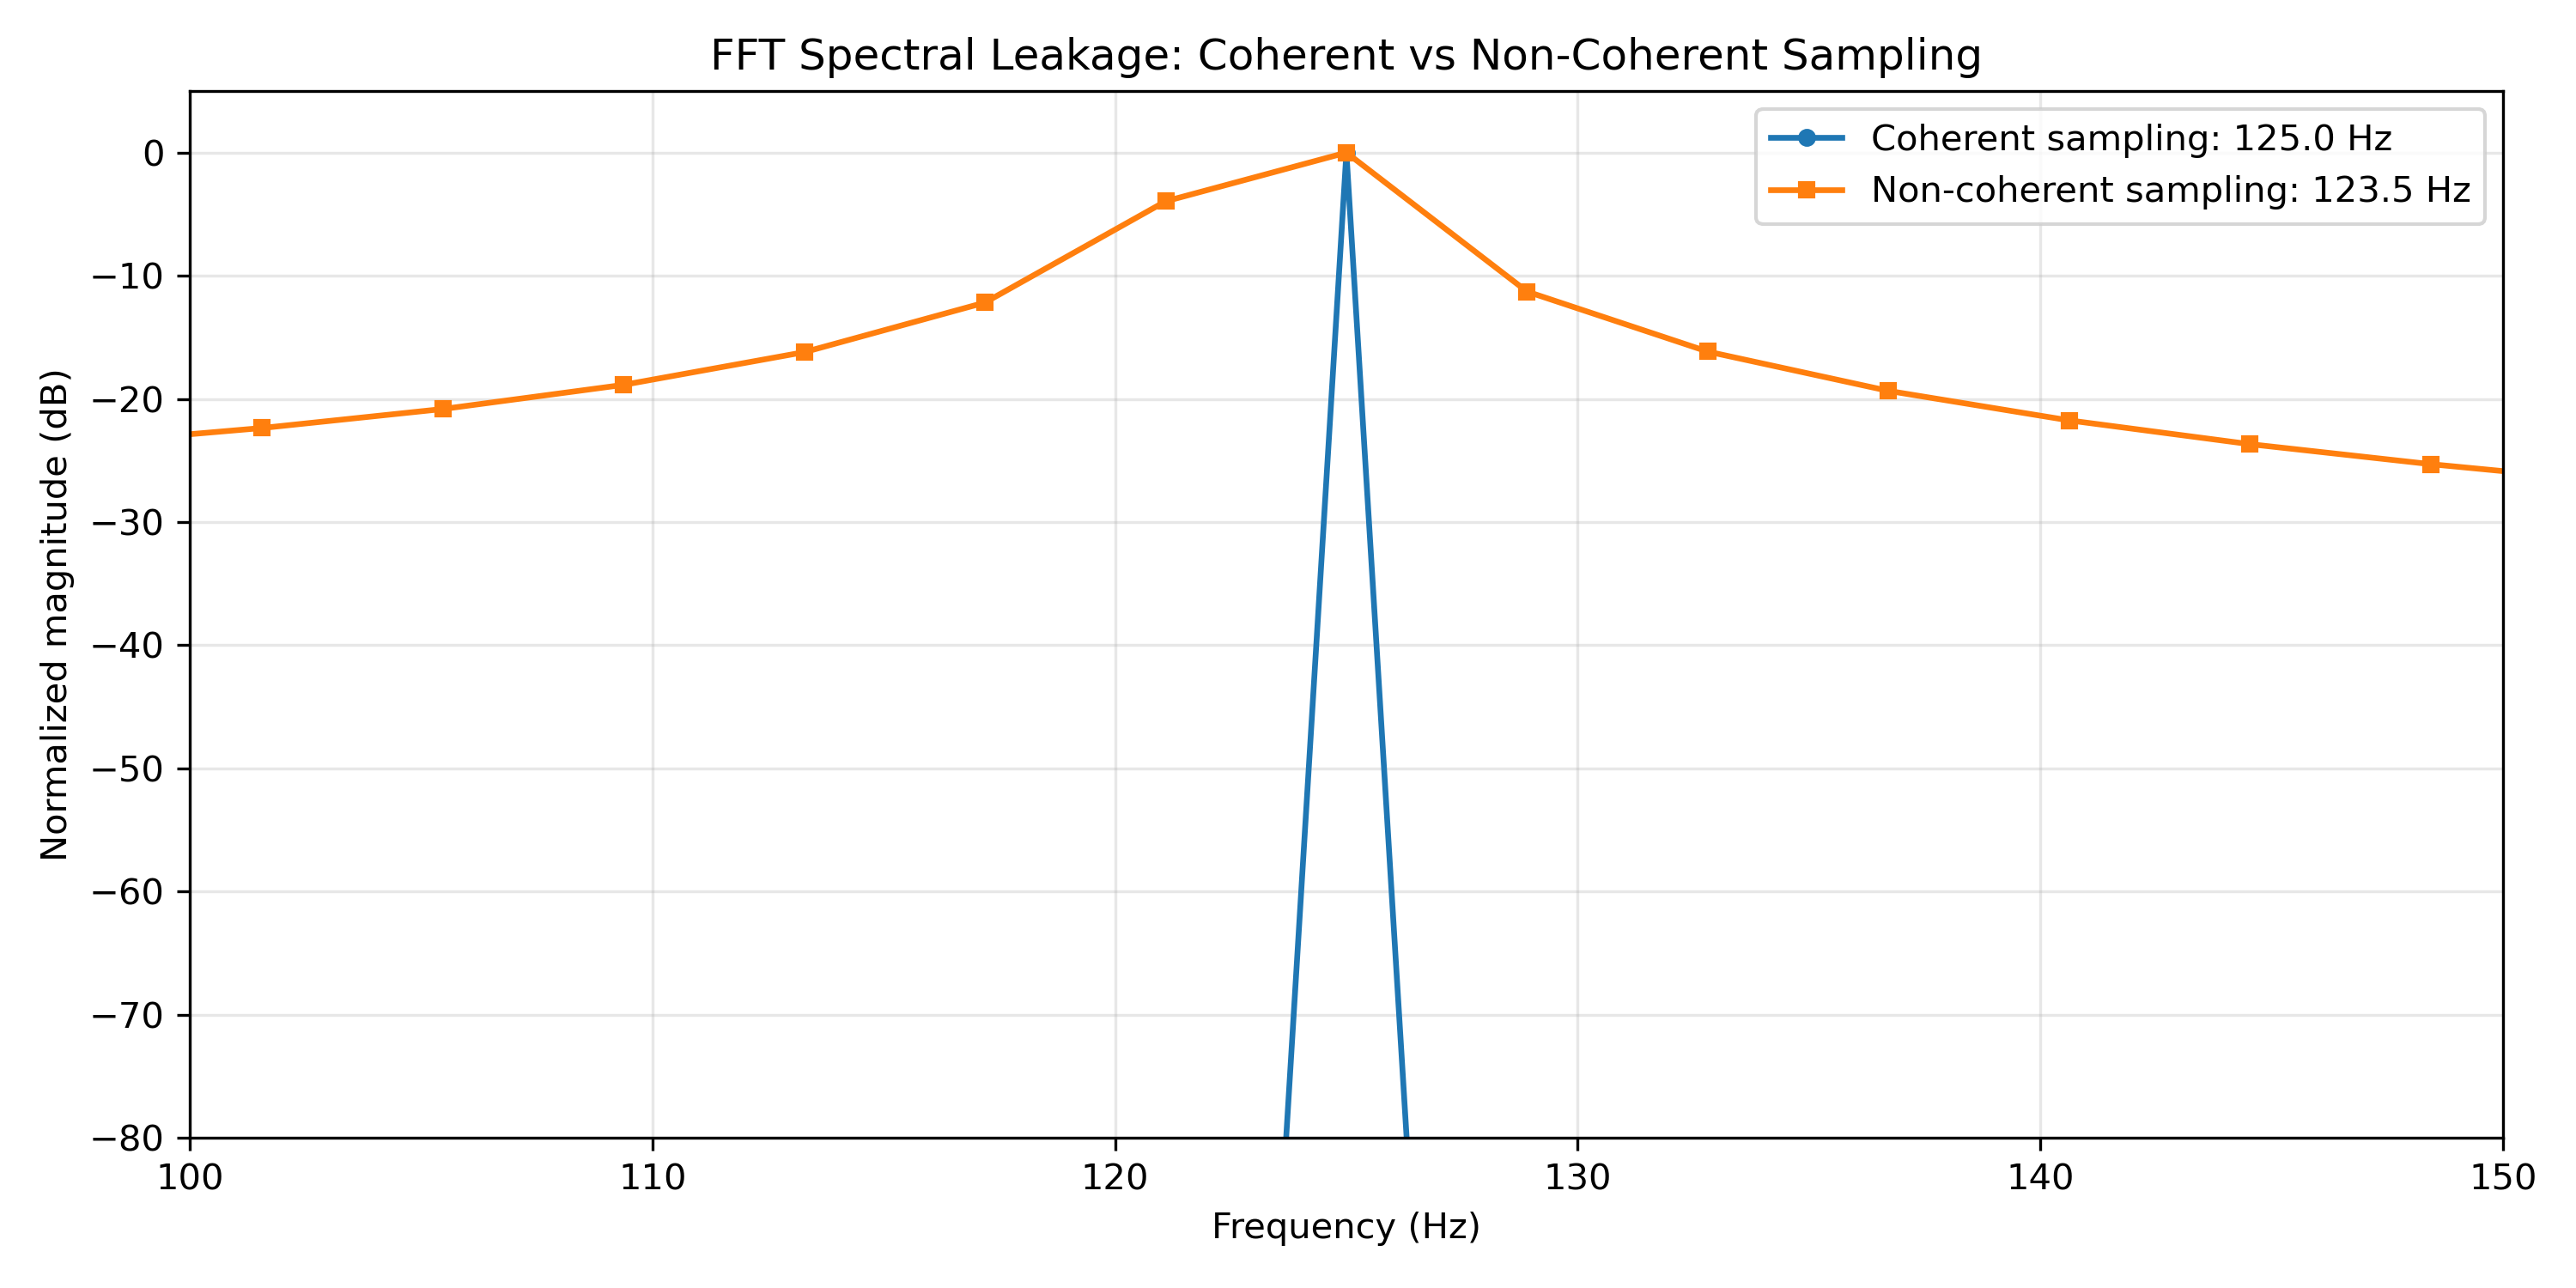
\includegraphics[width=0.92\linewidth]{../../python/ex01_fft_spectral_leakage/figures/fft_spectral_leakage.png}
}
{
\fbox{\parbox{0.85\linewidth}{Line-marker FFT figure not found. Run the Python script from the repository root to generate the FFT spectral leakage figure.}}
}
\caption{Zoomed line-marker FFT spectral leakage comparison between coherent and non-coherent sinusoidal sampling.}
\label{fig:fft_leakage_line_marker}
\end{figure}

\begin{figure}[htbp]
\centering
\IfFileExists{../../python/ex01_fft_spectral_leakage/figures/fft_spectral_leakage_stem.png}
{
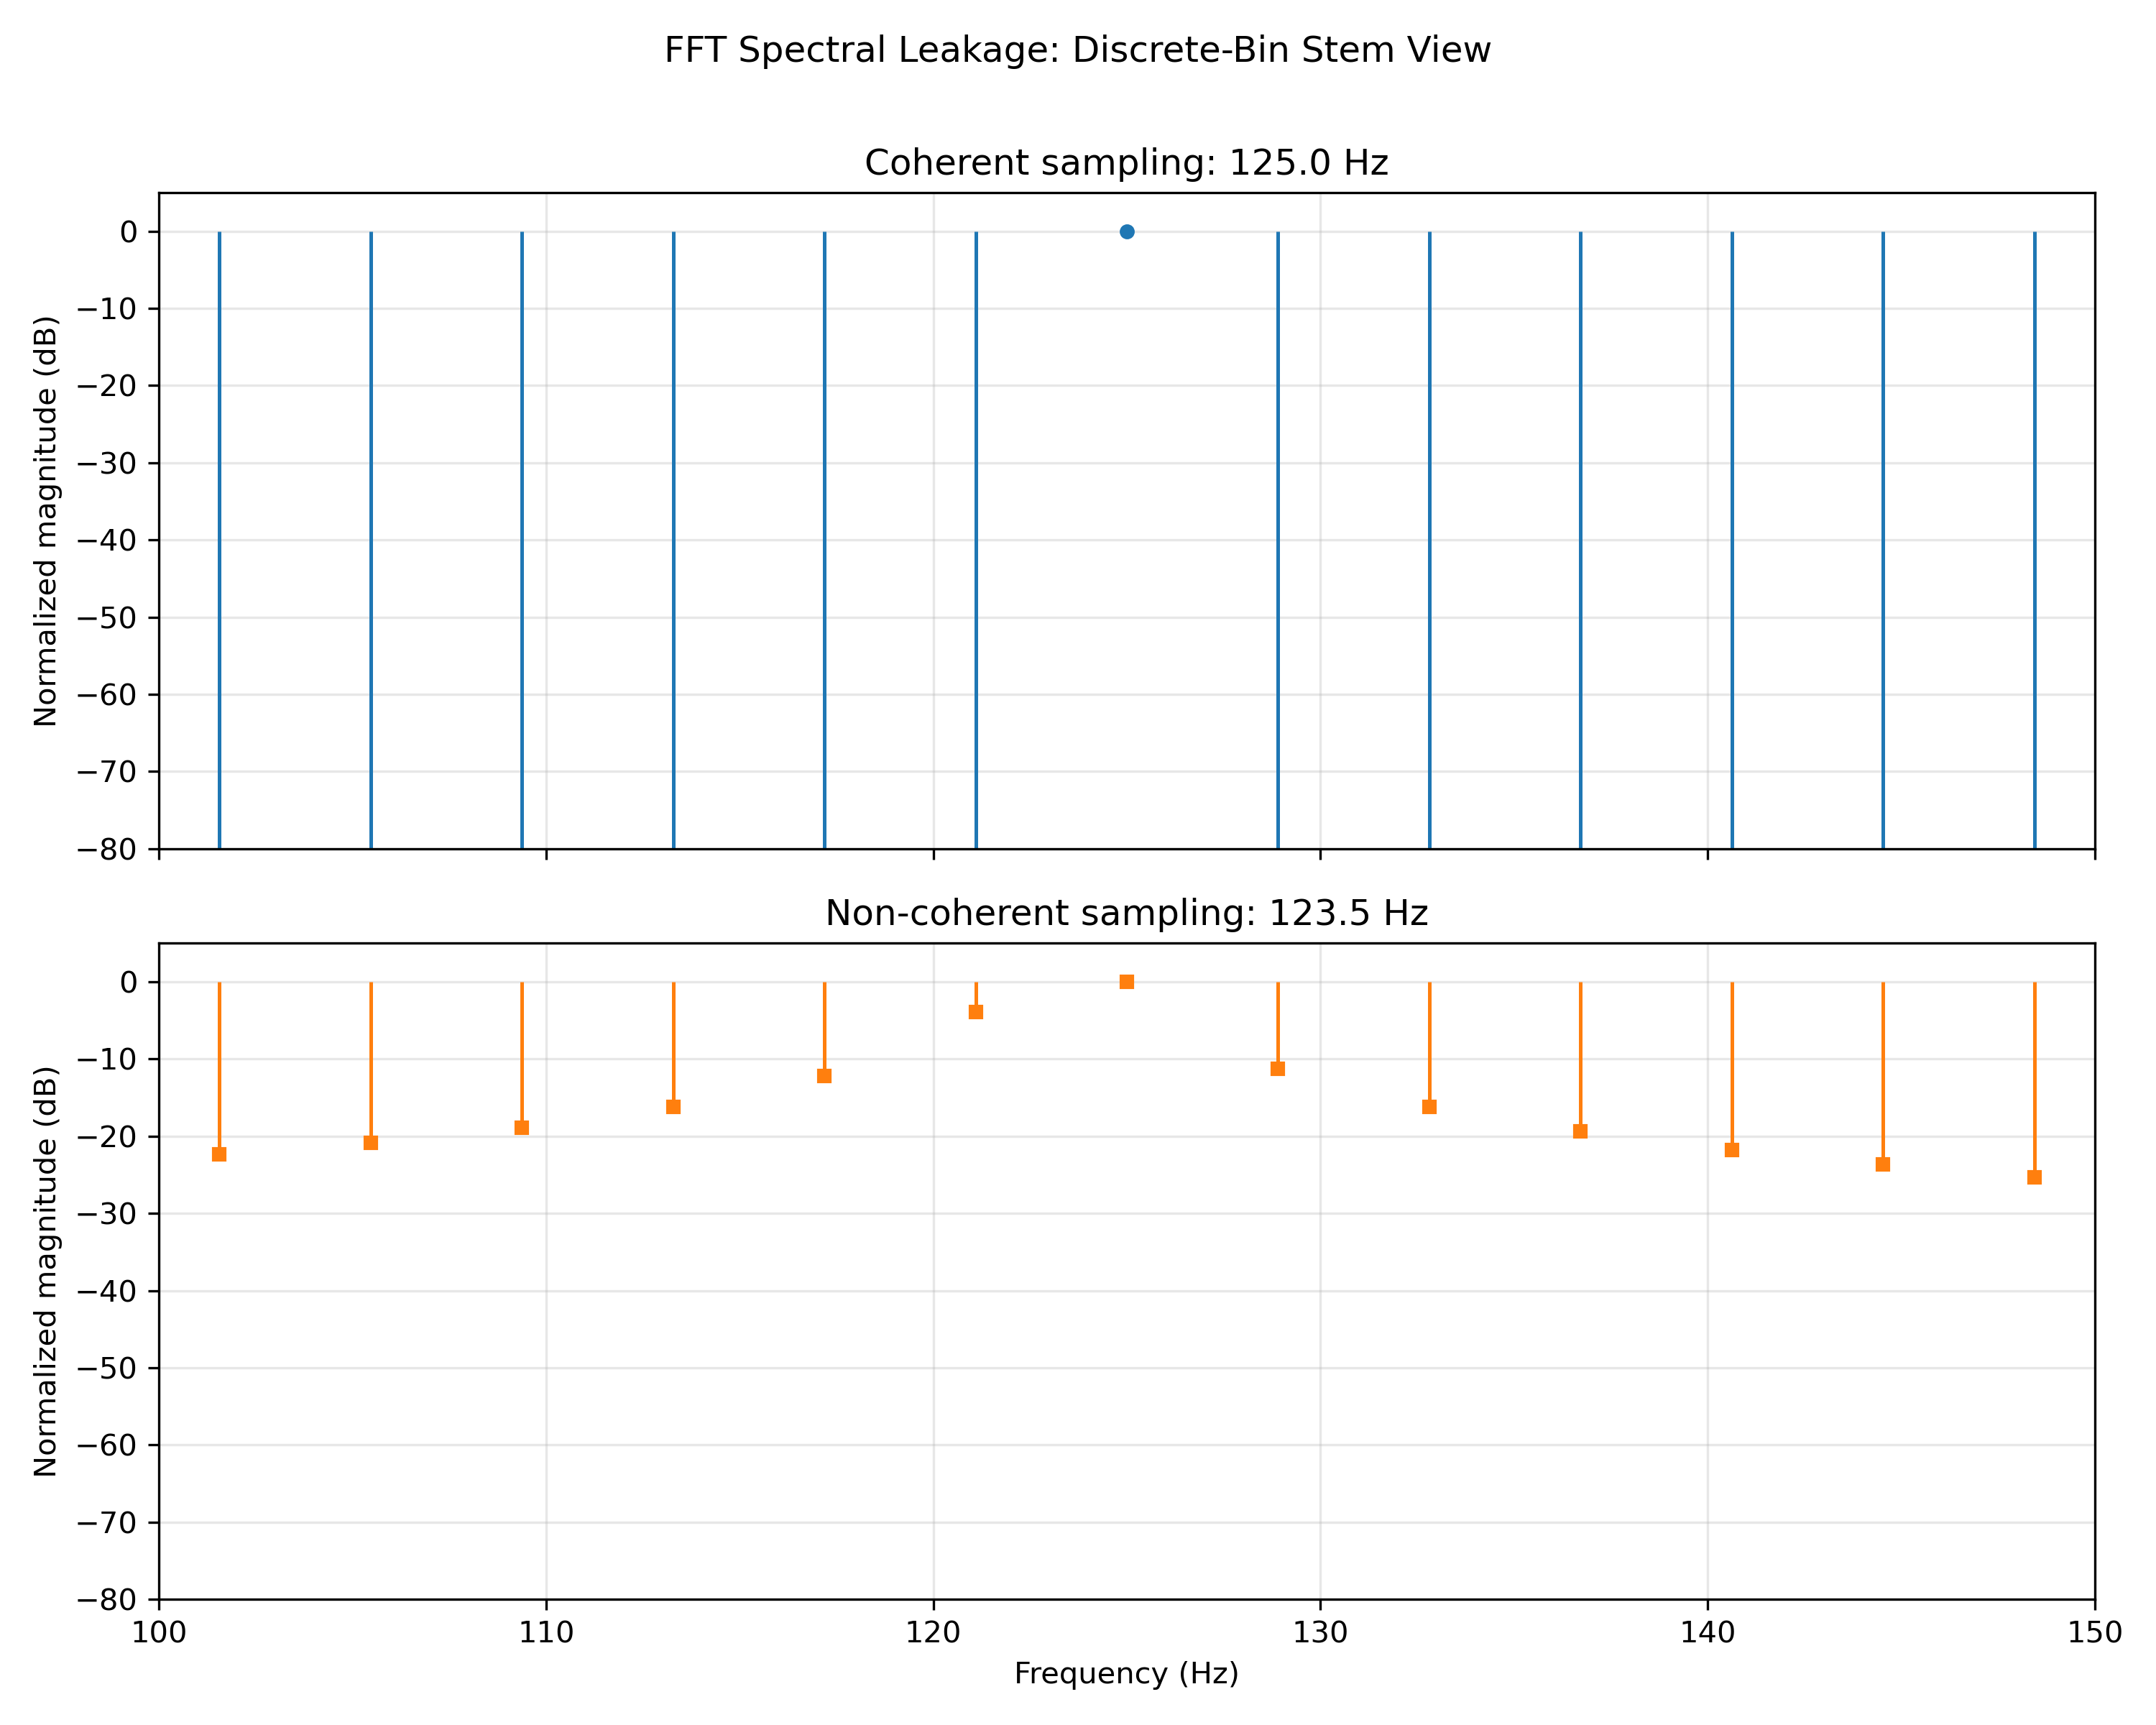
\includegraphics[width=0.92\linewidth]{../../python/ex01_fft_spectral_leakage/figures/fft_spectral_leakage_stem.png}
}
{
\fbox{\parbox{0.85\linewidth}{Stem FFT figure not found. Run the Python script from the repository root to generate the FFT spectral leakage stem figure.}}
}
\caption{Stacked stem-plot view of the coherent and non-coherent FFT spectra, emphasizing the discrete-bin nature of the FFT.}
\label{fig:fft_leakage_stem}
\end{figure}
\section{Engineering Interpretation}

Spectral leakage is not an implementation defect. It is a consequence of finite-duration measurement and mismatch between the input frequency and the FFT analysis grid.

This effect matters in engineering systems because leakage can mask weak components, distort frequency estimates, and complicate interpretation of spectra. It is relevant in vibration monitoring, instrumentation, communications, radar Doppler processing, and array-processing pipelines.

For radar and array-processing workflows, the lesson is especially important: preprocessing decisions such as sampling duration, windowing, and spectral resolution can influence downstream covariance estimation, beamforming, and detection performance.

\section{Preparation for Exercise 02}

Exercise 01 uses the implicit rectangular window. Exercise 02 can extend this analysis by applying explicit window functions:

\begin{itemize}
\item Hann window,
\item Hamming window,
\item Blackman window.
\end{itemize}

The expected tradeoff is:

\begin{quote}
Windowing reduces sidelobe leakage but widens the main lobe.
\end{quote}

This tradeoff connects leakage suppression to frequency resolution.

\section{Conclusion}

The FFT represents a finite sampled signal using a discrete frequency basis. If the signal frequency aligns with a DFT basis vector, the spectrum is compact. If the signal frequency lies between basis vectors, the signal projects onto multiple DFT basis vectors and spectral leakage appears.

The matrix formulation makes the phenomenon clear: spectral leakage is a basis-mismatch effect in a finite-dimensional frequency representation. This viewpoint is useful not only for FFT exercises, but also for advanced DSP workflows involving spectral estimation, radar processing, beamforming, and DOA analysis.

\end{document}
